\documentclass[aspectratio=169]{beamer}
\mode<presentation>
\usetheme{Hannover}
\useoutertheme{sidebar}
\usecolortheme{dolphin}

\usepackage{amsmath}
\usepackage{amssymb}
\usepackage{enumerate}


% some bold math symbosl
\newcommand{\Cov}{\mathrm{Cov}}
\newcommand{\Cor}{\mathrm{Cor}}
\newcommand{\Var}{\mathrm{Var}}
\newcommand{\brho}{\boldsymbol{\rho}}
\newcommand{\bSigma}{\boldsymbol{\Sigma}}
\newcommand{\btheta}{\boldsymbol{\theta}}
\newcommand{\bbeta}{\boldsymbol{\beta}}
\newcommand{\bmu}{\boldsymbol{\mu}}
\newcommand{\bW}{\mathbf{W}}
\newcommand{\one}{\mathbf{1}}
\newcommand{\bH}{\mathbf{H}}
\newcommand{\by}{\mathbf{y}}
\newcommand{\bolde}{\mathbf{e}}
\newcommand{\bx}{\mathbf{x}}

\newcommand{\cpp}[1]{\texttt{#1}}

\title{Mathematical Biostatistics Bootcamp: Lecture 9, Confidence Intervals}
\author{Brian Caffo}
\date{\today}
\institute[Department of Biostatistics]{
  Department of Biostatistics \\
  Johns Hopkins Bloomberg School of Public Health\\
  Johns Hopkins University
}


\begin{document}

\frame{\titlepage}


\section{Table of contents}
\frame{
  \frametitle{Table of contents}
  \tableofcontents
}


\section{Confidence intervals}
\begin{frame}\frametitle{Confidence intervals}
  \begin{itemize}
  \item Previously, we discussed creating a confidence interval using the CLT
  \item Now we discuss the creation of better confidence intervals for small
    samples using Gosset's $t$ distribution
  \item To discuss the $t$ distribution we must discuss the Chi-squared
    distribution
  \item Throughout we use the following general procedure for creating CIs
    \begin{enumerate}[a.]
    \item Create a {\bf Pivot} or statistic that does not depend on the
      parameter of interest
    \item Solve the probability that the pivot lies between bounds for 
    the parameter
  \end{enumerate}
\end{itemize}
\end{frame}

\begin{frame}\frametitle{The Chi-squared distribution}
  \begin{itemize}
  \item Suppose that $S^2$ is the sample variance from a collection of iid
    $N(\mu,\sigma^2)$ data; then 
    $$
    \frac{(n - 1) S^2}{\sigma^2} \sim \chi^2_{n-1}
    $$
    which reads: follows a Chi-squared distribution with $n-1$ degrees of freedom
  \item The Chi-squared distribution is skewed and has support on $0$ to $\infty$
  \item The mean of the Chi-squared is its degrees of freedom 
  \item The variance of the Chi-squared distribution is twice the degrees of freedom
  \end{itemize}
\end{frame}

\section{CI for a normal variance}
\begin{frame}\frametitle{Confidence interval for the variance} 
Note that if $\chi^2_{n-1, \alpha}$ is the $\alpha$ quantile of the
Chi-squared distribution then
\begin{eqnarray*}
  1 - \alpha & = & P \left( \chi^2_{n-1, \alpha/2} \leq  \frac{(n - 1) S^2}{\sigma^2} \leq  \chi^2_{n-1,1 - \alpha/2} \right) \\ \\
& = &  P\left(\frac{(n-1)S^2}{\chi^2_{n-1,1-\alpha/2}} \leq \sigma^2 \leq 
\frac{(n-1)S^2}{\chi^2_{n-1,\alpha/2}} \right) \\
\end{eqnarray*}
So that 
$$
\left[\frac{(n-1)S^2}{\chi^2_{n-1,1-\alpha/2}}, \frac{(n-1)S^2}{\chi^2_{n-1,\alpha/2}}\right]
$$ \ \\ \ \\
is a $100(1-\alpha)\%$ confidence interval for $\sigma^2$
\end{frame}

\begin{frame}\frametitle{Notes about this interval}
\begin{itemize}
\item This interval relies heavily on the assumed normality
\item Square-rooting the endpoints yields a CI for $\sigma$
\item It turns out that  
$$
(n - 1)S^2 \sim \mbox{Gamma}\{(n-1)/2, 2\sigma^2\}
$$
which reads: follows a gamma distribution with shape $(n-1)/2$ and scale
$2\sigma^2$
\item Therefore, this can be used to plot a likelihood function for
  $\sigma^2$
\end{itemize}
\end{frame}

\begin{frame}\frametitle{Example}
\begin{itemize}
\item A recent study 513 of organo-lead manufacturing workers reported
  an average total brain volume of $1,150.315$ $cm^3$ with a standard
  deviation of $105.977$. Assuming normality of the underlying
  measurements, calculate a confidence interval for the population
  variation in total brain volume.
\end{itemize}
\end{frame}

\begin{frame}[fragile]\frametitle{Example continued}
\begin{verbatim}
##CI for the variance
s2 <- 105.977 ^ 2
n <- 513
alpha <- .05
qtiles <- qchisq(c(alpha/2, 1 - alpha/2), 
                 n - 1)
ival <- rev((n - 1) * s2 / qtiles)
##interval for the sd
sqrt(ival)
[1]  99.86484 112.89216
\end{verbatim}
\end{frame}

\begin{frame}[fragile]\frametitle{Plot the likelihood}
\begin{verbatim}
sigmaVals <- seq(90, 120, length = 1000)
likeVals <- dgamma((n - 1) * s2,
                   shape = (n - 1)/2,
                   scale = 2*sigmaVals^2)
likeVals <- likeVals / max(likeVals)
plot(sigmaVals, likeVals, type = "l")
lines(range(sigmaVals[likeVals >= 1 / 8]), 
      c(1 / 8, 1 / 8))
lines(range(sigmaVals[likeVals >= 1 / 16]), 
      c(1 / 16, 1 / 16))
\end{verbatim}
\end{frame}


\begin{frame}
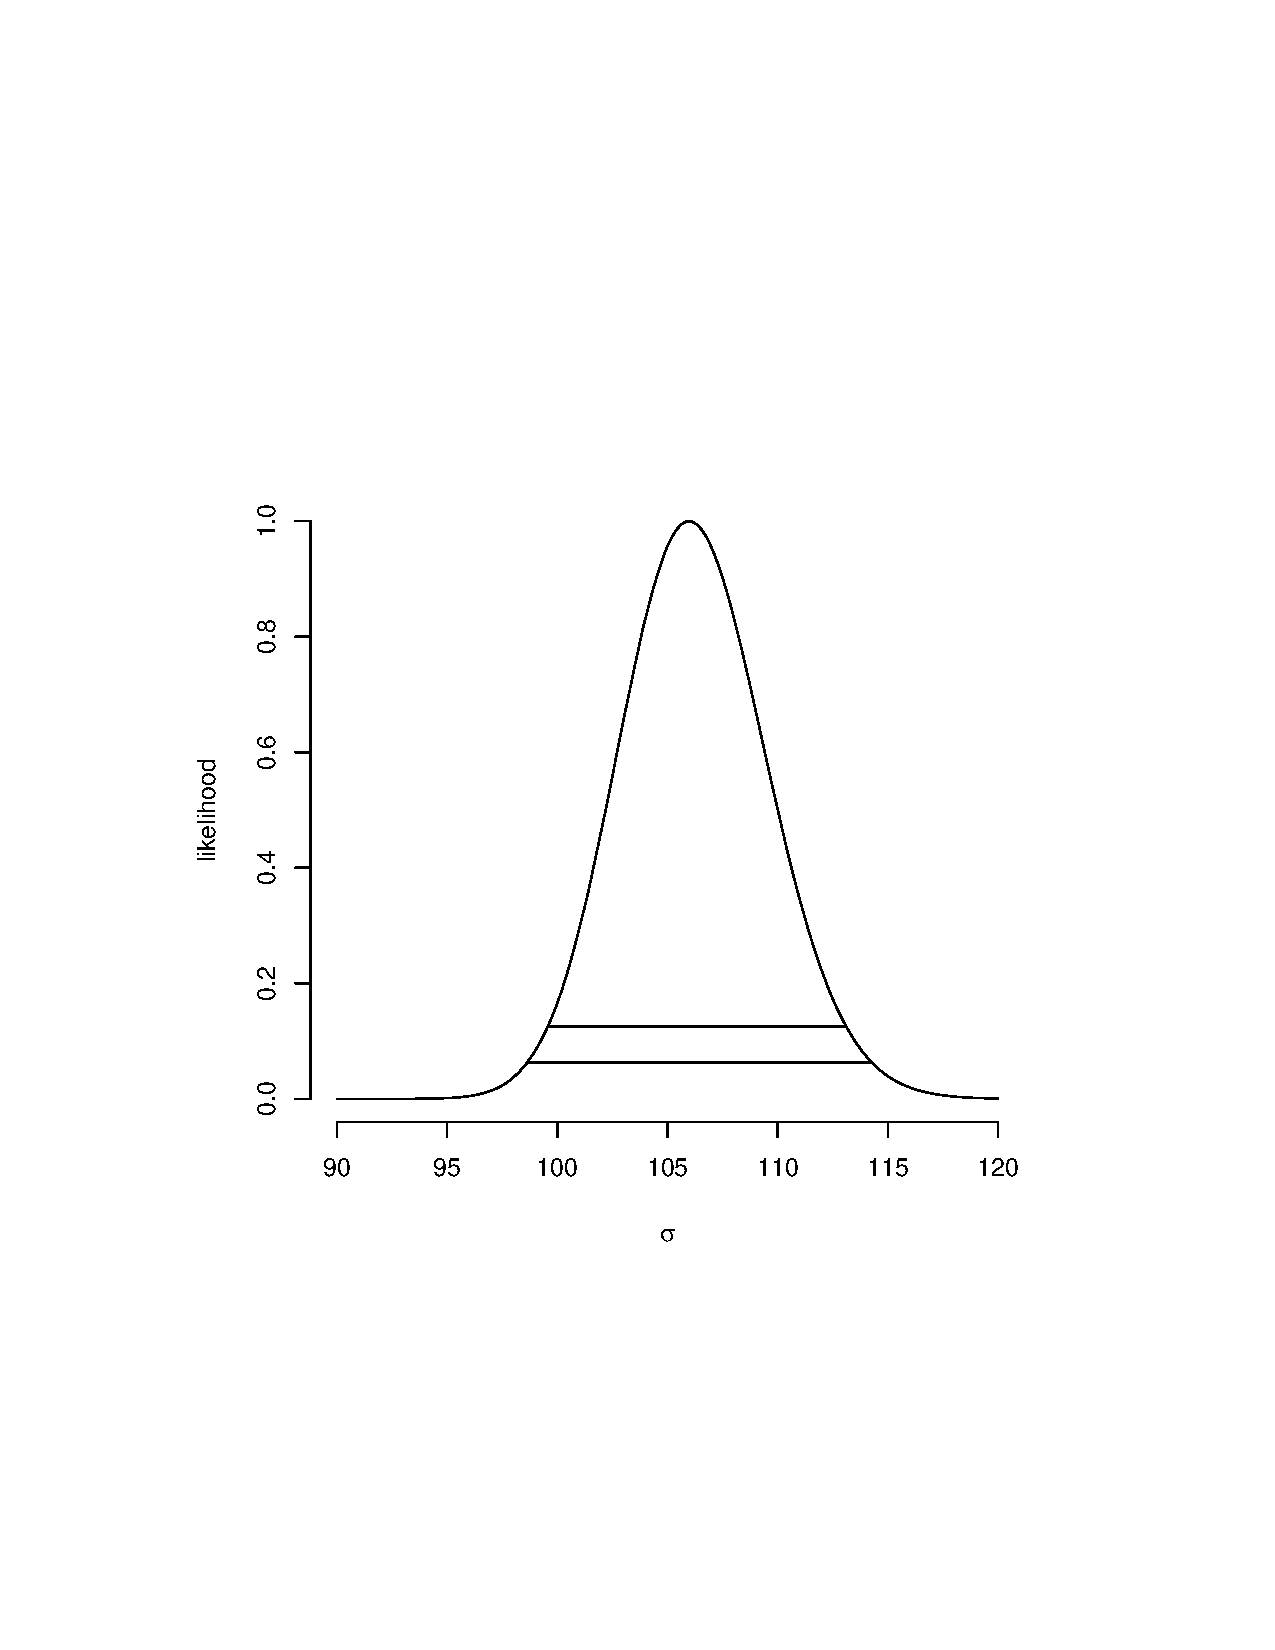
\includegraphics[width=3.5in]{varianceLikelihood.pdf}
\end{frame}

\section{Student's $t$ distribution}
\begin{frame}\frametitle{Gosset's $t$ distribution}
\begin{itemize}
\item Invented by William Gosset (under the pseudonym ``Student'') in 1908
\item Has thicker tails than the normal
\item Is indexed by a degrees of freedom; gets more like a standard
  normal as df gets larger
\item Is obtained as 
$$
\frac{Z}{\sqrt{\frac{\chi^2}{df}}}
$$
where $Z$ and $\chi^2$ are independent standard normals and
Chi-squared distributions respectively
\end{itemize}
\end{frame}

\begin{frame}\frametitle{Result}
\begin{itemize}
\item Suppose that $(X_1,\ldots,X_n)$ are iid $N(\mu,\sigma^2)$,
  then:
  \begin{enumerate}[a.]
  \item $\frac{\bar X - \mu}{\sigma / \sqrt{n}}$ is standard normal
  \item $\sqrt{\frac{(n - 1) S^2}{\sigma^2 (n - 1)}} = S / \sigma$
    is the square root of a Chi-squared divided by its df
  \end{enumerate}
  \item Therefore 
    $$
\frac{\frac{\bar X - \mu}{\sigma /\sqrt{n}}}{S/\sigma}  
= \frac{\bar X - \mu}{S/\sqrt{n}}
    $$
    follows Gosset's $t$ distribution with $n-1$ degrees of freedom
\end{itemize}
\end{frame}

\section{Confidence intervals for normal means}
\begin{frame}\frametitle{Confidence intervals for the mean}
\begin{itemize}
\item Notice that the $t$ statistic is a pivot, therefore we use it
  to create a confidence interval for $\mu$
\item Let $t_{df,\alpha}$ be the $\alpha^{th}$ quantile of the t distribution with
  $df$ degrees of freedom
  \begin{eqnarray*}
&   & 1 - \alpha \\
& = & P\left(-t_{n-1,1-\alpha/2} \leq \frac{\bar X - \mu}{S/\sqrt{n}} \leq t_{n-1,1-\alpha/2}\right) \\ \\
& = & P\left(\bar X - t_{n-1,1-\alpha/2} S / \sqrt{n} \leq \mu  
      \leq \bar X + t_{n-1,1-\alpha/2}S /\sqrt{n}\right)
  \end{eqnarray*}
\item Interval is $\bar X \pm t_{n-1,1-\alpha/2} S/\sqrt{n}$
\end{itemize}
\end{frame}

\begin{frame}\frametitle{Note's about the $t$ interval}
\begin{itemize}
\item The $t$ interval technically assumes that the data are iid normal,
  though it is robust to this assumption
\item It works well whenever the distribution of the data is roughly
  symmetric and mound shaped
\item Paired observations are often analyzed using the $t$ interval by
  taking differences
\item For large degrees of freedom, $t$ quantiles become the same as standard
  normal quantiles; therefore this interval converges to the same interval as
  the CLT yielded
\end{itemize}
\end{frame}

\begin{frame}
\begin{itemize}
\item For skewed distributions, the spirit of the $t$ interval
  assumptions are violated
\item Also, for skewed distributions, it doesn't make a lot of sense
  to center the interval at the mean
\item In this case, consider taking logs or using a different summary
  like the median
\item For highly discrete data, like binary, other intervals are available
\end{itemize}
\end{frame}

\begin{frame}\frametitle{Sleep data}
In R typing \texttt{data(sleep)} brings up the sleep data originally
analyzed in Gosset's Biometrika paper, which shows the increase in
hours for 10 patients on two soporific drugs. R treats the data as two
groups rather than paired.
\end{frame}

\begin{frame}[fragile]
\begin{verbatim}
Patient g1   g2  diff
1       0.7  1.9  1.2
2      -1.6  0.8  2.4
3      -0.2  1.1  1.3
4      -1.2  0.1  1.3
5      -0.1 -0.1  0.0
6       3.4  4.4  1.0
7       3.7  5.5  1.8
8       0.8  1.6  0.8
9       0.0  4.6  4.6
10      2.0  3.4  1.4
\end{verbatim}
\end{frame}

\begin{frame}[fragile]
\begin{verbatim}
data(sleep)
g1 <- sleep$extra[1 : 10]
g2 <- sleep$extra[11 : 20]
difference <- g2 - g1
mn <- mean(difference)#1.67
s <- sd(difference)#1.13
n <- 10
mn + c(-1, 1) * qt(.975, n-1) * s / sqrt(n)
t.test(difference)$conf.int
[1] 0.7001142 2.4598858
\end{verbatim}
\end{frame}

\begin{frame}\frametitle{The non-central $t$ distribution}
\begin{itemize}
\item If $X$ is $N(\mu,\sigma^2)$ and $\chi^2$ is a Chi-squared random
  variable with $df$ degrees of freedom then
  $\frac{X/\sigma}{\sqrt{\frac{\chi^2}{df}}}$ is called a {\bf
    non-central} $t$ random variable with non-centrality parameter
  $\mu/\sigma$
\item Note that
  \begin{enumerate}[a.]
  \item $\bar X$ is $N(\mu, \sigma^2/n)$
  \item $(n-1)S^2/\sigma^2$ is Chi-squared with $n-1$ df 
  \end{enumerate}
\item Then $\sqrt{n}\bar X / S$ is non-central $t$ with non-centrality
  parameter $\sqrt{n}\mu/\sigma$
\item We can use this to create a likelihood for $\mu/\sigma$, the {\bf effect size}
\end{itemize}
\end{frame}

\begin{frame}[fragile]\frametitle{Some code}
Starting after the code for the $t$ interval
\begin{verbatim}
tStat <- sqrt(n) * mn / s
esVals <- seq(0, 1, length = 1000)
likVals <- dt(tStat, n - 1, ncp = sqrt(n) * esVals)
likVals <- likVals / max(likVals)
plot(esVals, likVals, type = "l")
lines(range(esVals[likVals>1/8]), c(1/8,1/8))
lines(range(esVals[likVals>1/16]), c(1/16,1/16))
\end{verbatim}
\end{frame}

\begin{frame}
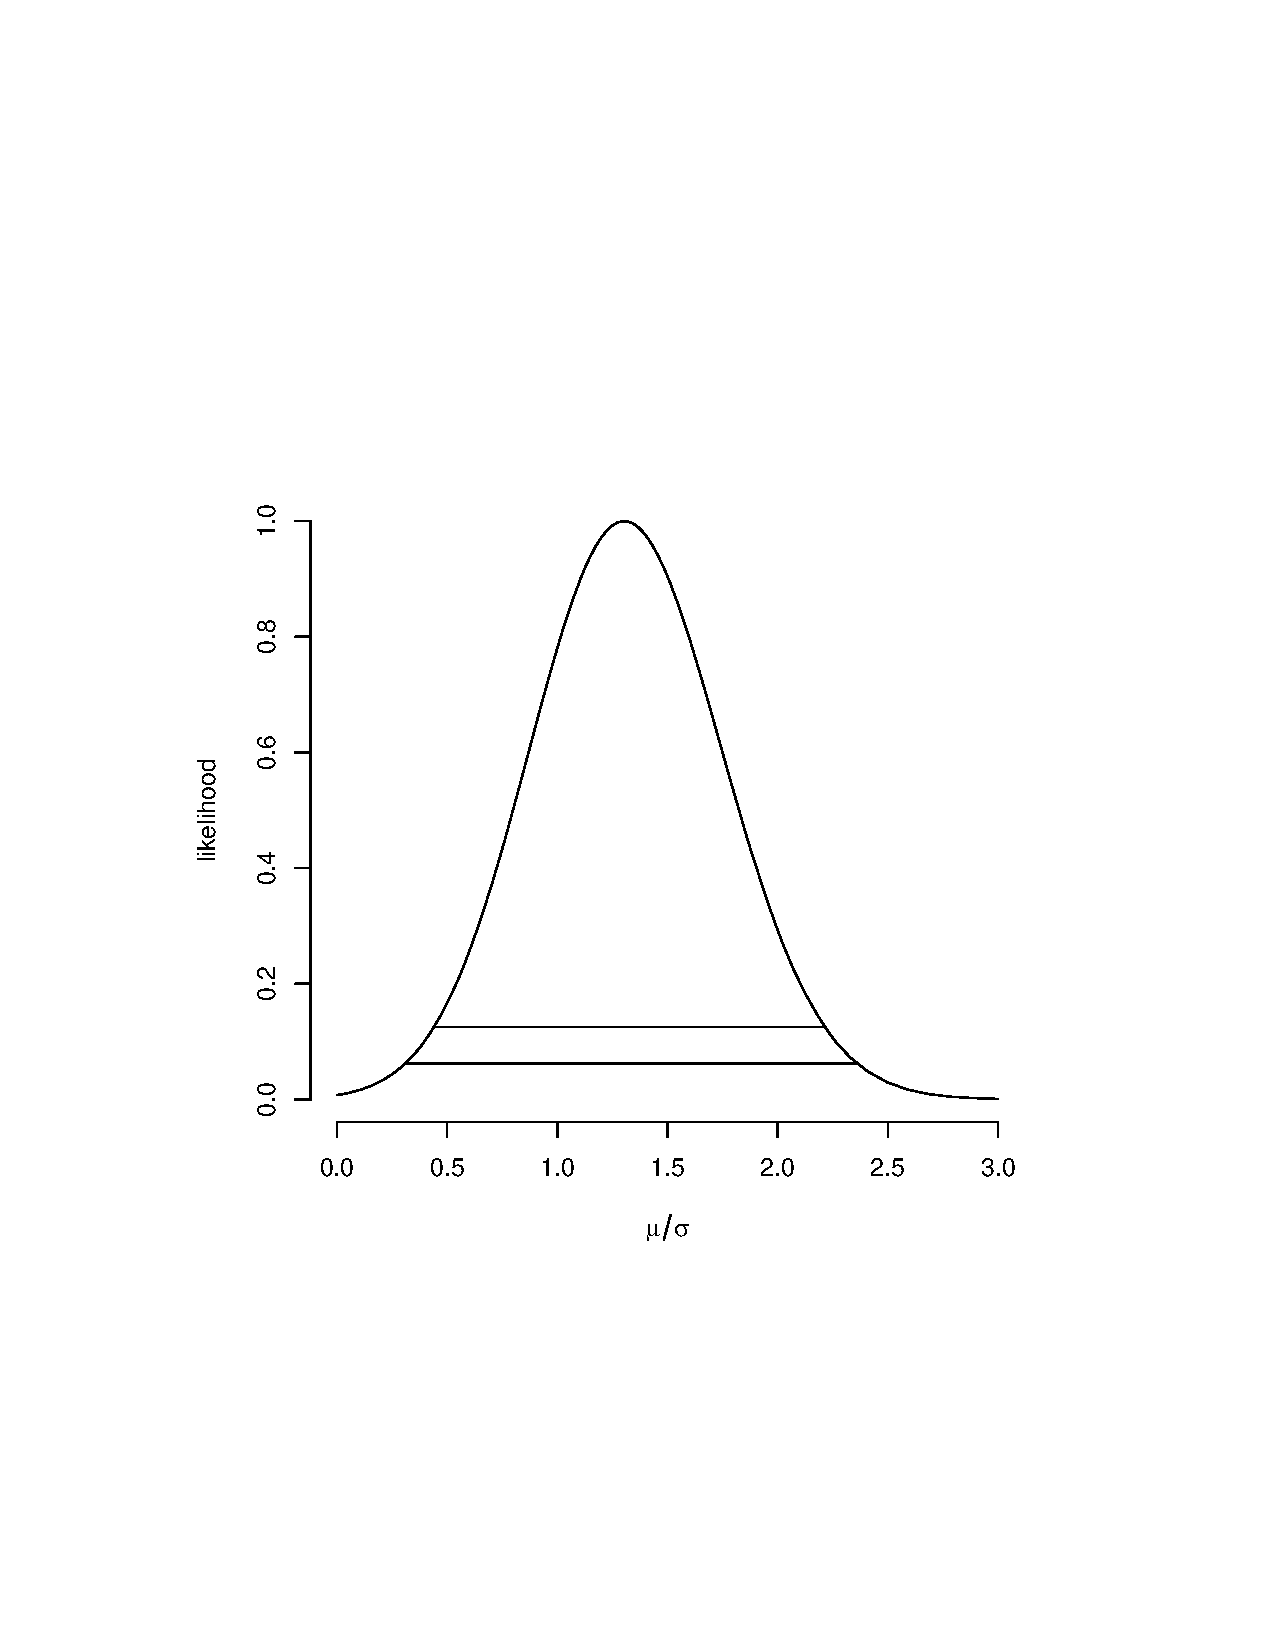
\includegraphics[width=3.5in]{normalLikelihoodMean.pdf}
\end{frame}

\section{Profile likelihoods}
\begin{frame}\frametitle{The profile likelihood}
\begin{itemize}
\item To obtain a likelihood for $\mu$ alone, the preferred method is called {\bf profiling}
\item The profile likelihood gets its name because the result is like the shadow you would
  get if you were to shine a light on the two-dimensional likelihood for $\mu$ and $\sigma$
\item The profile likelihood for parameter value $\mu_0$ is obtained by maximizing the
  joint likelihood for $\sigma$ with $\mu$ fixed at $\mu_0$
\item This process is repeated for lots of values of $\mu_0$
\end{itemize}
\end{frame}

\begin{frame}\frametitle{Calculating the profile likelihood}
\begin{itemize}
\item The joint likelihood with $\mu$ fixed at $\mu_0$ is
  \begin{eqnarray*}
& \propto &\prod_{i=1}^n \left[(\sigma^2)^{-1/2}\exp\left\{-(x_i - \mu_0)^2/2\sigma^2 \right\} \right]\\
& = &  (\sigma^2)^{-n/2}\exp\left\{-\sum_{i=1}^n(x_i - \mu_0)^2/2\sigma^2 \right\}
  \end{eqnarray*}
\item With $\mu_0$ fixed, the maximum likelihood estimator for $\sigma^2$ is
  $\sum_{i=1}^n(x_i - \mu_0)^2 / n$ (homework)
\item Plugging this back into the likelihood we get
$$
\left(\sum_{i=1}^n(x_i - \mu_0)^2 / n \right)^{-n/2}\exp(-n/2)
$$
\end{itemize}
\end{frame}

\begin{frame}\frametitle{Continued}
\begin{itemize}
\item Therefore, removing multiplicative constants, the profile likelihood is 
  $$
  \left(\sum_{i=1}^n(x_i - \mu)^2 \right)^{-n/2}
  $$
\item Note that this is clearly maximized at $\mu=\bar X$, the same as the ML
  estimate for $\mu$ for the complete likelihood
\end{itemize}
\end{frame}

\begin{frame}[fragile]\frametitle{Some code}
\begin{verbatim}
muVals <- seq(0, 3, length = 1000)
likVals <- sapply(muVals,
                  function(mu){
                    (sum((difference-mu)^2) /
                     sum((difference-mn)^2))^(-n/2) 
                  }
                  )
plot(muVals, likVals, type = "l")
lines(range(muVals[likVals>1/8]), c(1/8,1/8))
lines(range(muVals[likVals>1/16]), c(1/16,1/16))
\end{verbatim}
\end{frame}

\begin{frame}
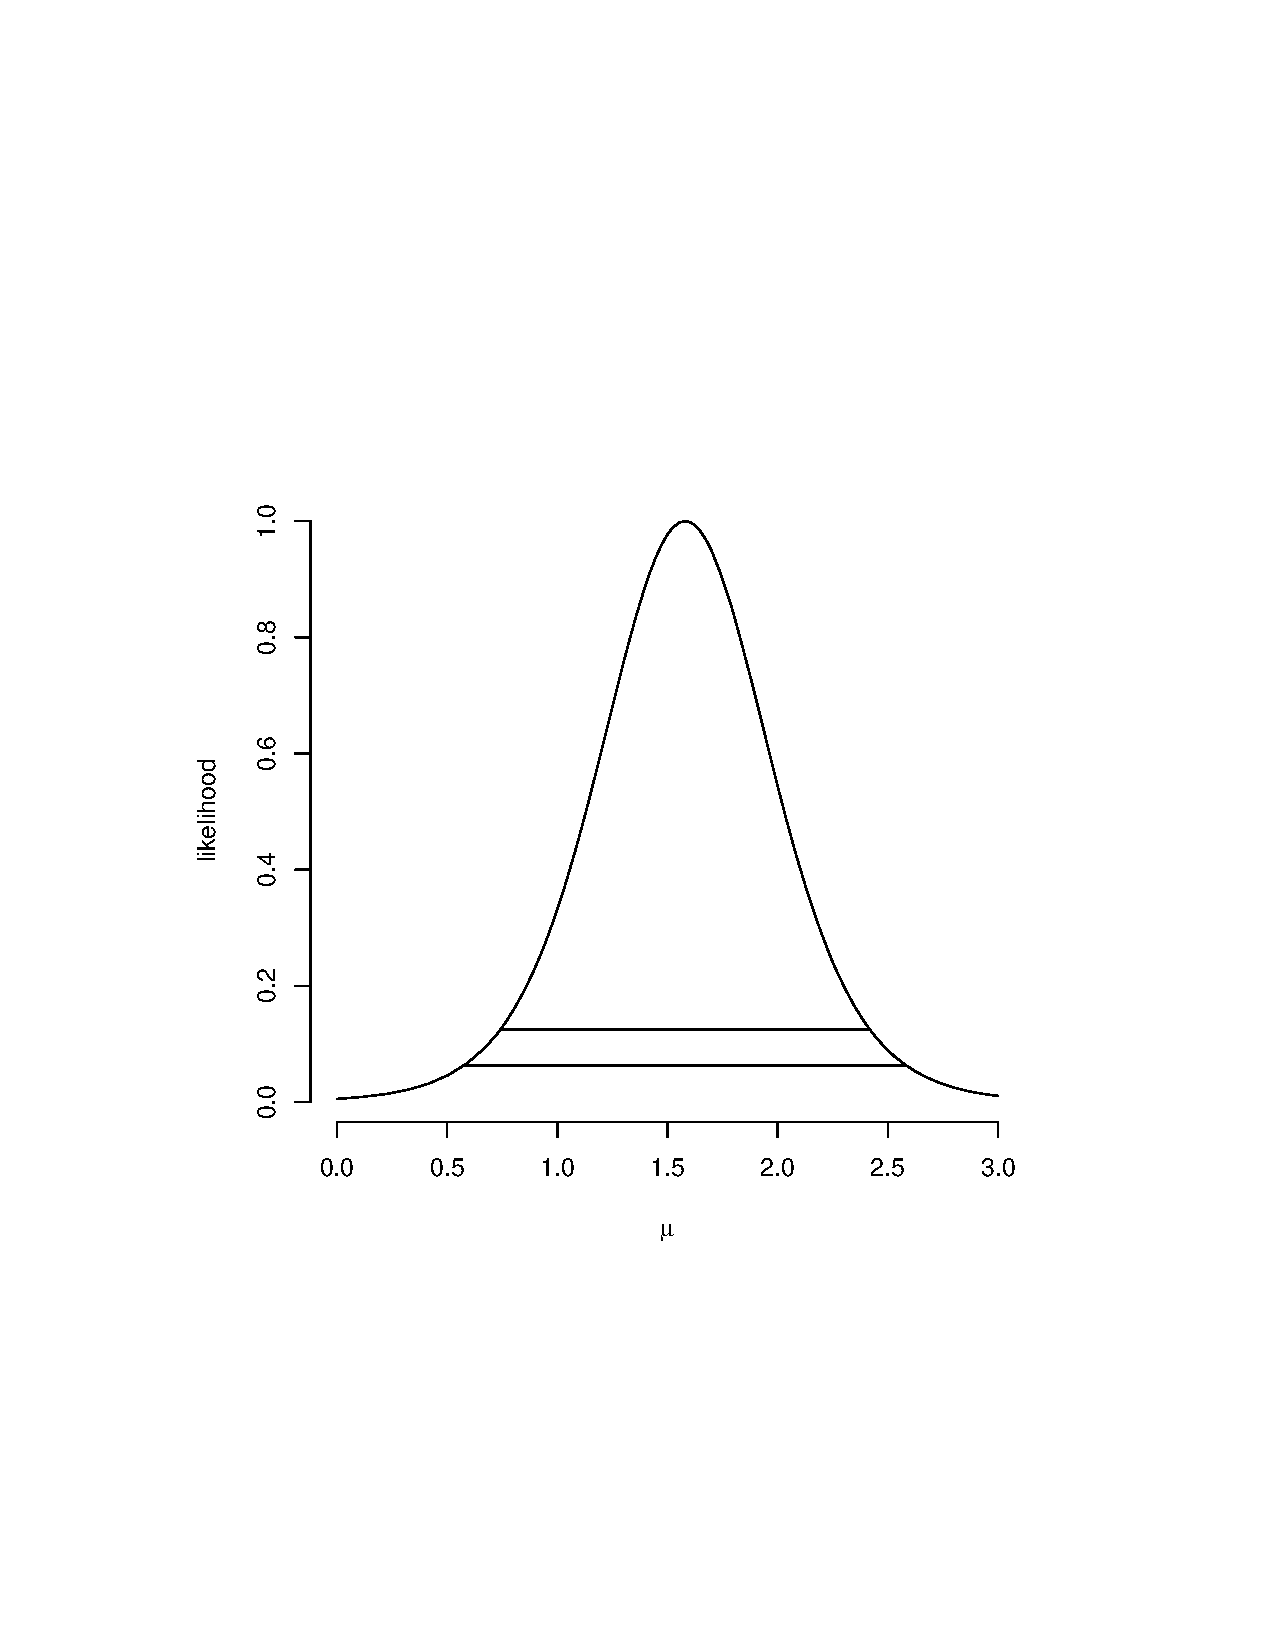
\includegraphics[width=3.5in]{normalProfileLikelihoodMean.pdf}
\end{frame}

\end{document}

